%% Extended Data for "The energy productivity of neighbourhood form".
%% Standalone document; compiles to extended_data.pdf and accompanies
%% main.tex at submission. Numbers match paper/results_snapshot.txt
%% (regenerated 2026-07-10). Figures built by stats/argument_figures.py
%% and stats/map_figures.py.

\documentclass[pdflatex,sn-nature]{sn-jnl}

\usepackage{graphicx}
\usepackage{amsmath,amssymb,amsfonts}
\usepackage{booktabs}

\graphicspath{{../figures/}}

% Generated by the stats scripts via stats/ledger.py — do not edit.
% Regenerate by running the stats scripts (see paper/submission_checklist.md).
\newcommand{\nepialphaEightGap}{2.93}
\newcommand{\nepialphaEightGapCI}{2.72--3.15}
\newcommand{\nepialphaSixGap}{2.80}
\newcommand{\nepialphaSixGapCI}{2.62--2.99}
\newcommand{\nepialphaZeroGap}{2.50}
\newcommand{\nepialphaZeroGapCI}{2.35--2.65}
\newcommand{\nepicatchAmen}{1.26}
\newcommand{\nepicatchAmenCI}{1.05--1.51}
\newcommand{\nepicatchJobs}{1.67}
\newcommand{\nepicatchJobsCI}{1.30--2.15}
\newcommand{\nepicatchPeople}{1.17}
\newcommand{\nepicatchPeopleCI}{0.99--1.38}
\newcommand{\nepicccClosed}{16}
\newcommand{\nepicccGap}{1.89}
\newcommand{\nepicccGapCI}{1.80--1.98}
\newcommand{\nepicccSurvives}{84}
\newcommand{\nepiclusters}{309}
\newcommand{\nepicommuteSweepHi}{2.98}
\newcommand{\nepicommuteSweepLo}{2.74}
\newcommand{\nepicopHigh}{1.89}
\newcommand{\nepicopLow}{1.88}
\newcommand{\nepicopMid}{1.89}
\newcommand{\nepidriveAmen}{11.3}
\newcommand{\nepidriveAmenCI}{8.2--15.5}
\newcommand{\nepidriveAmenRound}{11}
\newcommand{\nepidriveJobs}{14.3}
\newcommand{\nepidriveJobsCI}{10.2--20.1}
\newcommand{\nepidrivePeople}{11.1}
\newcommand{\nepidrivePeopleCI}{8.0--15.5}
\newcommand{\nepielecHeat}{1.55}
\newcommand{\nepievClosed}{18}
\newcommand{\nepievGap}{1.85}
\newcommand{\nepievGapCI}{1.72--1.99}
\newcommand{\nepifabricClosed}{20}
\newcommand{\nepifabricEvGap}{1.51}
\newcommand{\nepifabricEvGapCI}{1.43--1.59}
\newcommand{\nepifabricFactorMedian}{0.50}
\newcommand{\nepifabricGap}{1.83}
\newcommand{\nepifabricGapCI}{1.75--1.91}
\newcommand{\nepifamNowGap}{1.71}
\newcommand{\nepifloorElast}{0.54}
\newcommand{\nepifullClosed}{31}
\newcommand{\nepifullDetKwh}{9,600}
\newcommand{\nepifullFamDetKwh}{9,000}
\newcommand{\nepifullFamFlatKwh}{6,600}
\newcommand{\nepifullFamGap}{1.35}
\newcommand{\nepifullFamGapCI}{1.29--1.42}
\newcommand{\nepifullFamGapSd}{1.6}
\newcommand{\nepifullFamPremiumHundredK}{0.2}
\newcommand{\nepifullFamPremiumKwh}{2,300}
\newcommand{\nepifullFlatKwh}{5,700}
\newcommand{\nepifullGap}{1.68}
\newcommand{\nepifullGapCI}{1.62--1.74}
\newcommand{\nepifullGapSd}{2.5}
\newcommand{\nepifullPremiumHundredK}{0.4}
\newcommand{\nepifullPremiumKwh}{3,900}
\newcommand{\nepifullSurvives}{69}
\newcommand{\nepigasCovHeat}{1.61}
\newcommand{\nepigasCovTotal}{1.74}
\newcommand{\nepiheatFamGap}{1.27}
\newcommand{\nepiheatFamGapCI}{1.15--1.40}
\newcommand{\nepiheatGap}{1.60}
\newcommand{\nepiheatGapCI}{1.45--1.76}
\newcommand{\nepiheatSizeGap}{1.17}
\newcommand{\nepiheatSizeGapCI}{1.06--1.30}
\newcommand{\nepihhElast}{0.5}
\newcommand{\nepihpDelta}{2}
\newcommand{\nepihpGap}{2.16}
\newcommand{\nepihpGapCI}{2.08--2.25}
\newcommand{\nepiimdAccessRatio}{3.9}
\newcommand{\nepiimdEnergyRatio}{1.6}
\newcommand{\nepiimdRhoBristol}{-0.27}
\newcommand{\nepiimdRhoCambridge}{-0.33}
\newcommand{\nepiimdRhoInner}{-0.04}
\newcommand{\nepiimdRhoManchester}{-0.24}
\newcommand{\nepiimdRhoNat}{0.40}
\newcommand{\nepiimdRhoOxford}{-0.38}
\newcommand{\nepimSqGap}{0.92}
\newcommand{\nepimaupMedLsoa}{1.59}
\newcommand{\nepimaupMedMsoa}{1.47}
\newcommand{\nepimaupMedOa}{1.74}
\newcommand{\nepimaupTotalLsoa}{1.88}
\newcommand{\nepimaupTotalMsoa}{1.72}
\newcommand{\nepimaupTotalOa}{2.12}
\newcommand{\nepimedShare}{66}
\newcommand{\nepimedShareCI}{54--85}
\newcommand{\nepimeterDet}{0.94}
\newcommand{\nepimeterFlat}{0.81}
\newcommand{\nepimixBalanceAccess}{1.00}
\newcommand{\nepimixBalanceEnergy}{1.02}
\newcommand{\nepimixBalanceHi}{0.87}
\newcommand{\nepimixBalanceLo}{0.16}
\newcommand{\nepimixBalanceRate}{0.98}
\newcommand{\nepimixBalanceRateOa}{1.07}
\newcommand{\nepiosterBetaAdjTotal}{1.03}
\newcommand{\nepiosterDeltaHeat}{0.3}
\newcommand{\nepiosterDeltaTotal}{1.1}
\newcommand{\nepipopDensityDet}{14}
\newcommand{\nepipopDensityFlat}{79}
\newcommand{\nepipopDensityRatio}{5.7}
\newcommand{\nepiptAssumedTotal}{1.99}
\newcommand{\nepiptAssumedTotalCI}{1.90--2.10}
\newcommand{\nepiptAssumedTravel}{2.55}
\newcommand{\nepiptAssumedTravelCI}{2.40--2.71}
\newcommand{\nepiptBaseTotal}{2.12}
\newcommand{\nepiptCeilingTotal}{1.84}
\newcommand{\nepiptCeilingTotalCI}{1.74--1.93}
\newcommand{\nepiptCeilingTravel}{2.13}
\newcommand{\nepiptCeilingTravelCI}{2.00--2.26}
\newcommand{\nepiptClassAssumedTotal}{2.07}
\newcommand{\nepiptClassCeilingTotal}{1.98}
\newcommand{\nepiptIntensityAssumed}{0.35}
\newcommand{\nepiptRailShare}{73}
\newcommand{\nepiptSampleN}{178,347}
\newcommand{\nepirate}{3.9}
\newcommand{\nepirateCI}{3.1--4.8}
\newcommand{\nepirateCirc}{2.3}
\newcommand{\nepirateCircCI}{2.0--2.7}
\newcommand{\nepirateDomMedian}{3.0}
\newcommand{\nepirateHarm}{5.3}
\newcommand{\nepirateHarmCI}{4.2--6.7}
\newcommand{\nepisampleN}{178,353}
\newcommand{\nepiscenarioBase}{2.12}
\newcommand{\nepiscenarioBaseCI}{2.01--2.24}
\newcommand{\nepiscenarioN}{178,341}
\newcommand{\nepispatialBlockGap}{2.12}
\newcommand{\nepispatialBlockGapCI}{1.89--2.38}
\newcommand{\nepistockFamPremiumTwh}{14}
\newcommand{\nepistockPremiumShare}{21}
\newcommand{\nepistockPremiumTwh}{36}
\newcommand{\nepitotalGap}{2.12}
\newcommand{\nepitotalGapCI}{2.01--2.24}
\newcommand{\nepitotalGapRound}{2.1}
\newcommand{\nepitransitAdv}{4.3}
\newcommand{\nepitransitAdvCI}{3.6--5.2}
\newcommand{\nepitravelEv}{0.32}
\newcommand{\nepitravelFamGap}{2.68}
\newcommand{\nepitravelFamGapCI}{2.41--2.97}
\newcommand{\nepitravelGap}{3.07}
\newcommand{\nepitravelGapCI}{2.81--3.35}
\newcommand{\nepitravelIce}{0.93}
\newcommand{\nepitripHighAdv}{1.28}
\newcommand{\nepitripHighRate}{3.9}
\newcommand{\nepitripLowAdv}{1.37}
\newcommand{\nepitripLowRate}{4.2}
\newcommand{\nepitripMidAdv}{1.26}
\newcommand{\nepitripMidRate}{3.9}
\newcommand{\nepiwalkAmen}{27.2}
\newcommand{\nepiwalkAmenCI}{19.4--38.1}
\newcommand{\nepiwalkAmenDomMed}{9.7}
\newcommand{\nepiwalkAmenRound}{27}
\newcommand{\nepiwalkAmenSupport}{12.2}
\newcommand{\nepiwalkJobs}{52.4}
\newcommand{\nepiwalkJobsCI}{30.0--91.6}
\newcommand{\nepiwalkPeople}{12.5}
\newcommand{\nepiwalkPeopleCI}{9.4--16.5}
\newcommand{\nepiwinsorHeat}{1.59}
\newcommand{\nepiwithinSpread}{1.25}
\newcommand{\nepiwithinSpreadFam}{1.22}


\renewcommand{\figurename}{Extended Data Fig.}
\renewcommand{\tablename}{Extended Data Table}

\begin{document}

\title[Extended Data]{Extended Data: The energy productivity of neighbourhood form}

\author*[1]{\fnm{Gareth} \sur{Simons}}\email{gareth@benchmarkurbanism.com}
\affil*[1]{\orgdiv{Building Stock Lab, UCL Energy Institute}, \orgname{University College London}, \orgaddress{\city{London}, \country{United Kingdom}}}

\maketitle

\begin{figure}[p]
\centering
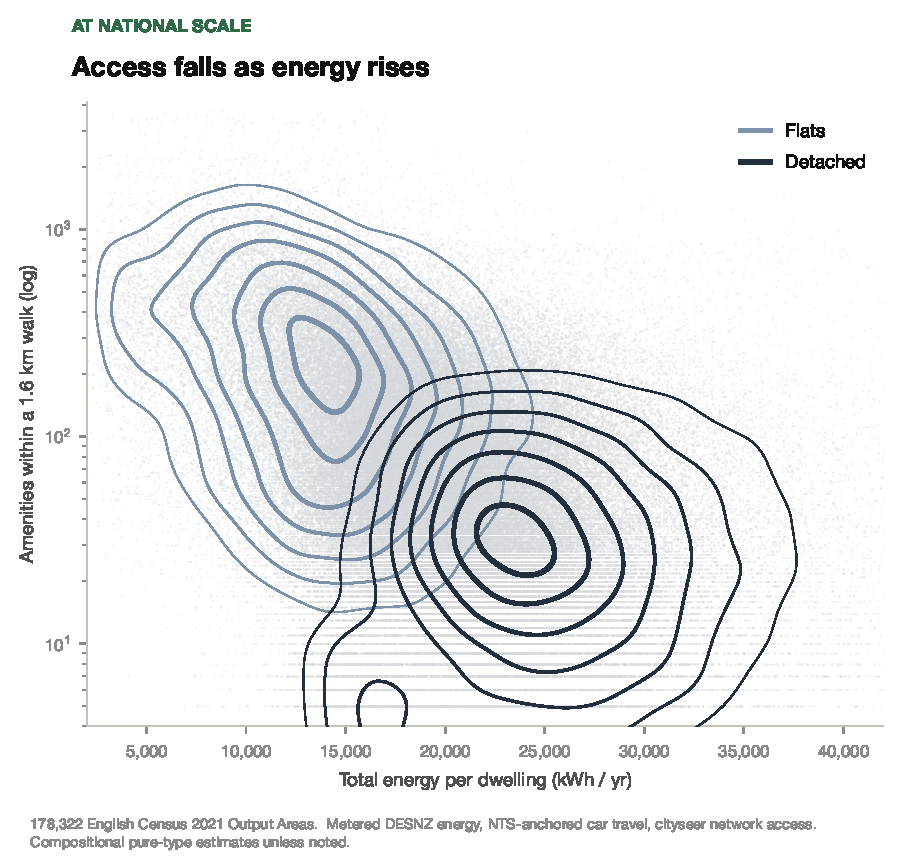
\includegraphics[width=\textwidth]{fig2_country}
\caption{\textbf{The joint distribution across all areas.} Every English Output Area is plotted by total energy per dwelling against amenities reachable on foot, as a hexagonal-bin density with a binned median line. Median access falls as energy per dwelling rises; the markers locate the median flat-dominant and detached-dominant areas.}
\label{edfig:country}
\end{figure}

\begin{figure}[p]
\centering
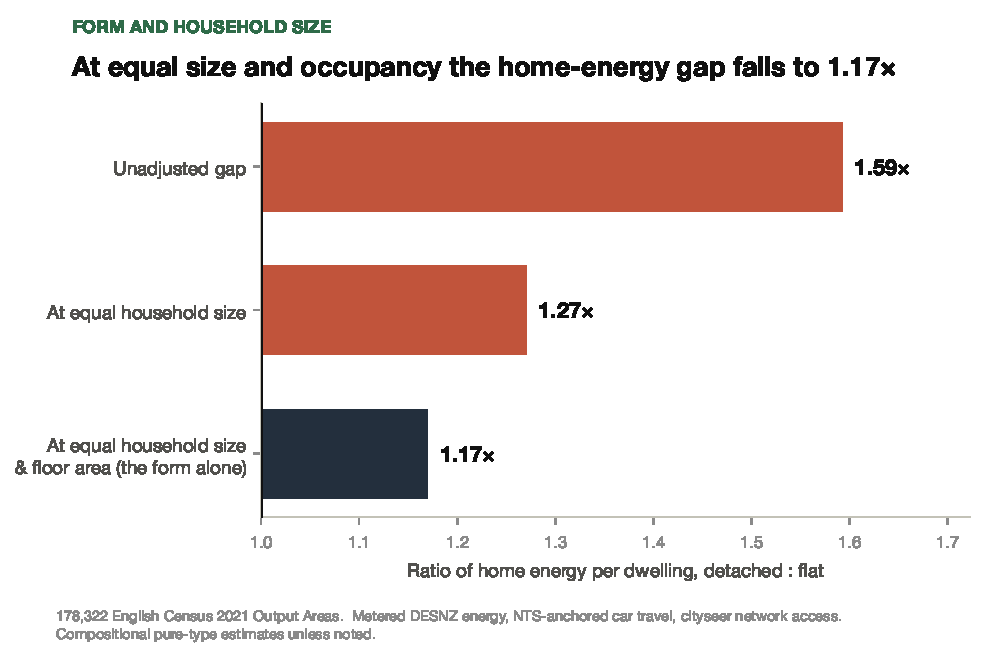
\includegraphics[width=\textwidth]{fig4_decomposition}
\caption{\textbf{Decomposition of the home-energy gap.} The compositional detached:flat home-energy contrast falls from \nepiheatGap$\times$ (95\% CI \nepiheatGapCI) to \nepiheatFamGap$\times$ (\nepiheatFamGapCI) at equal household size and to \nepiheatSizeGap$\times$ (\nepiheatSizeGapCI) at equal floor area; on the log scale, size and occupancy account for \nepimedShare\% (\nepimedShareCI\%) of the gap. The decomposition is a covariate adjustment on cross-sectional data, not an identified mediation.}
\label{edfig:decomposition}
\end{figure}

\begin{figure}[p]
\centering
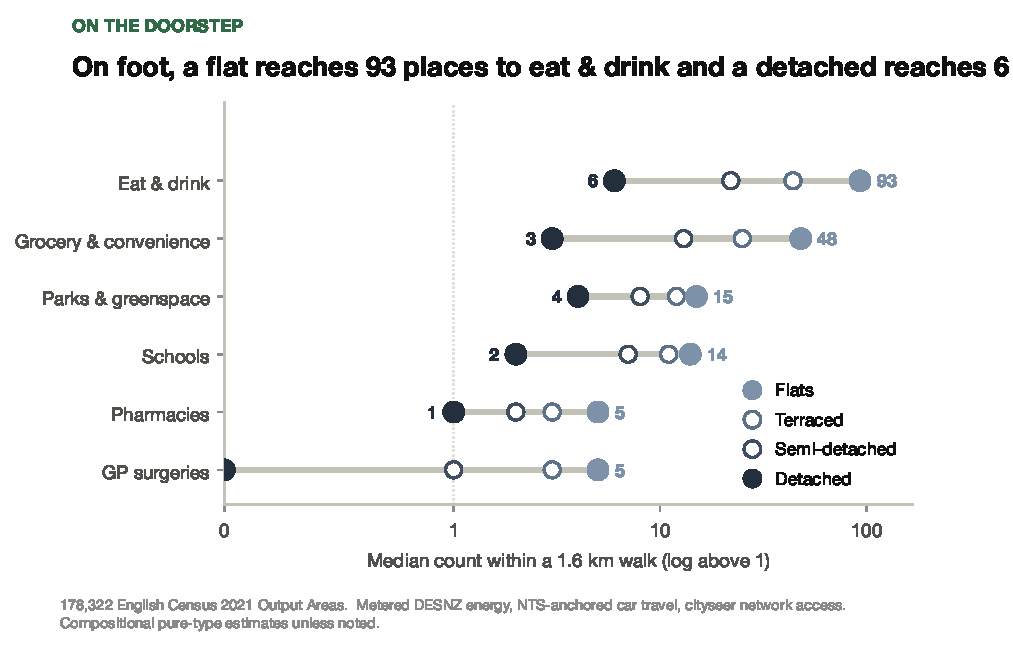
\includegraphics[width=\textwidth]{fig5_doorstep}
\caption{\textbf{Per-service counts at walking distance.} Median counts within a 1.6\,km network walk are shown by service for flat-dominant and detached-dominant areas. The median detached-dominant area has no general practitioner within the 1.6\,km walk.}
\label{edfig:doorstep}
\end{figure}

\begin{figure}[p]
\centering
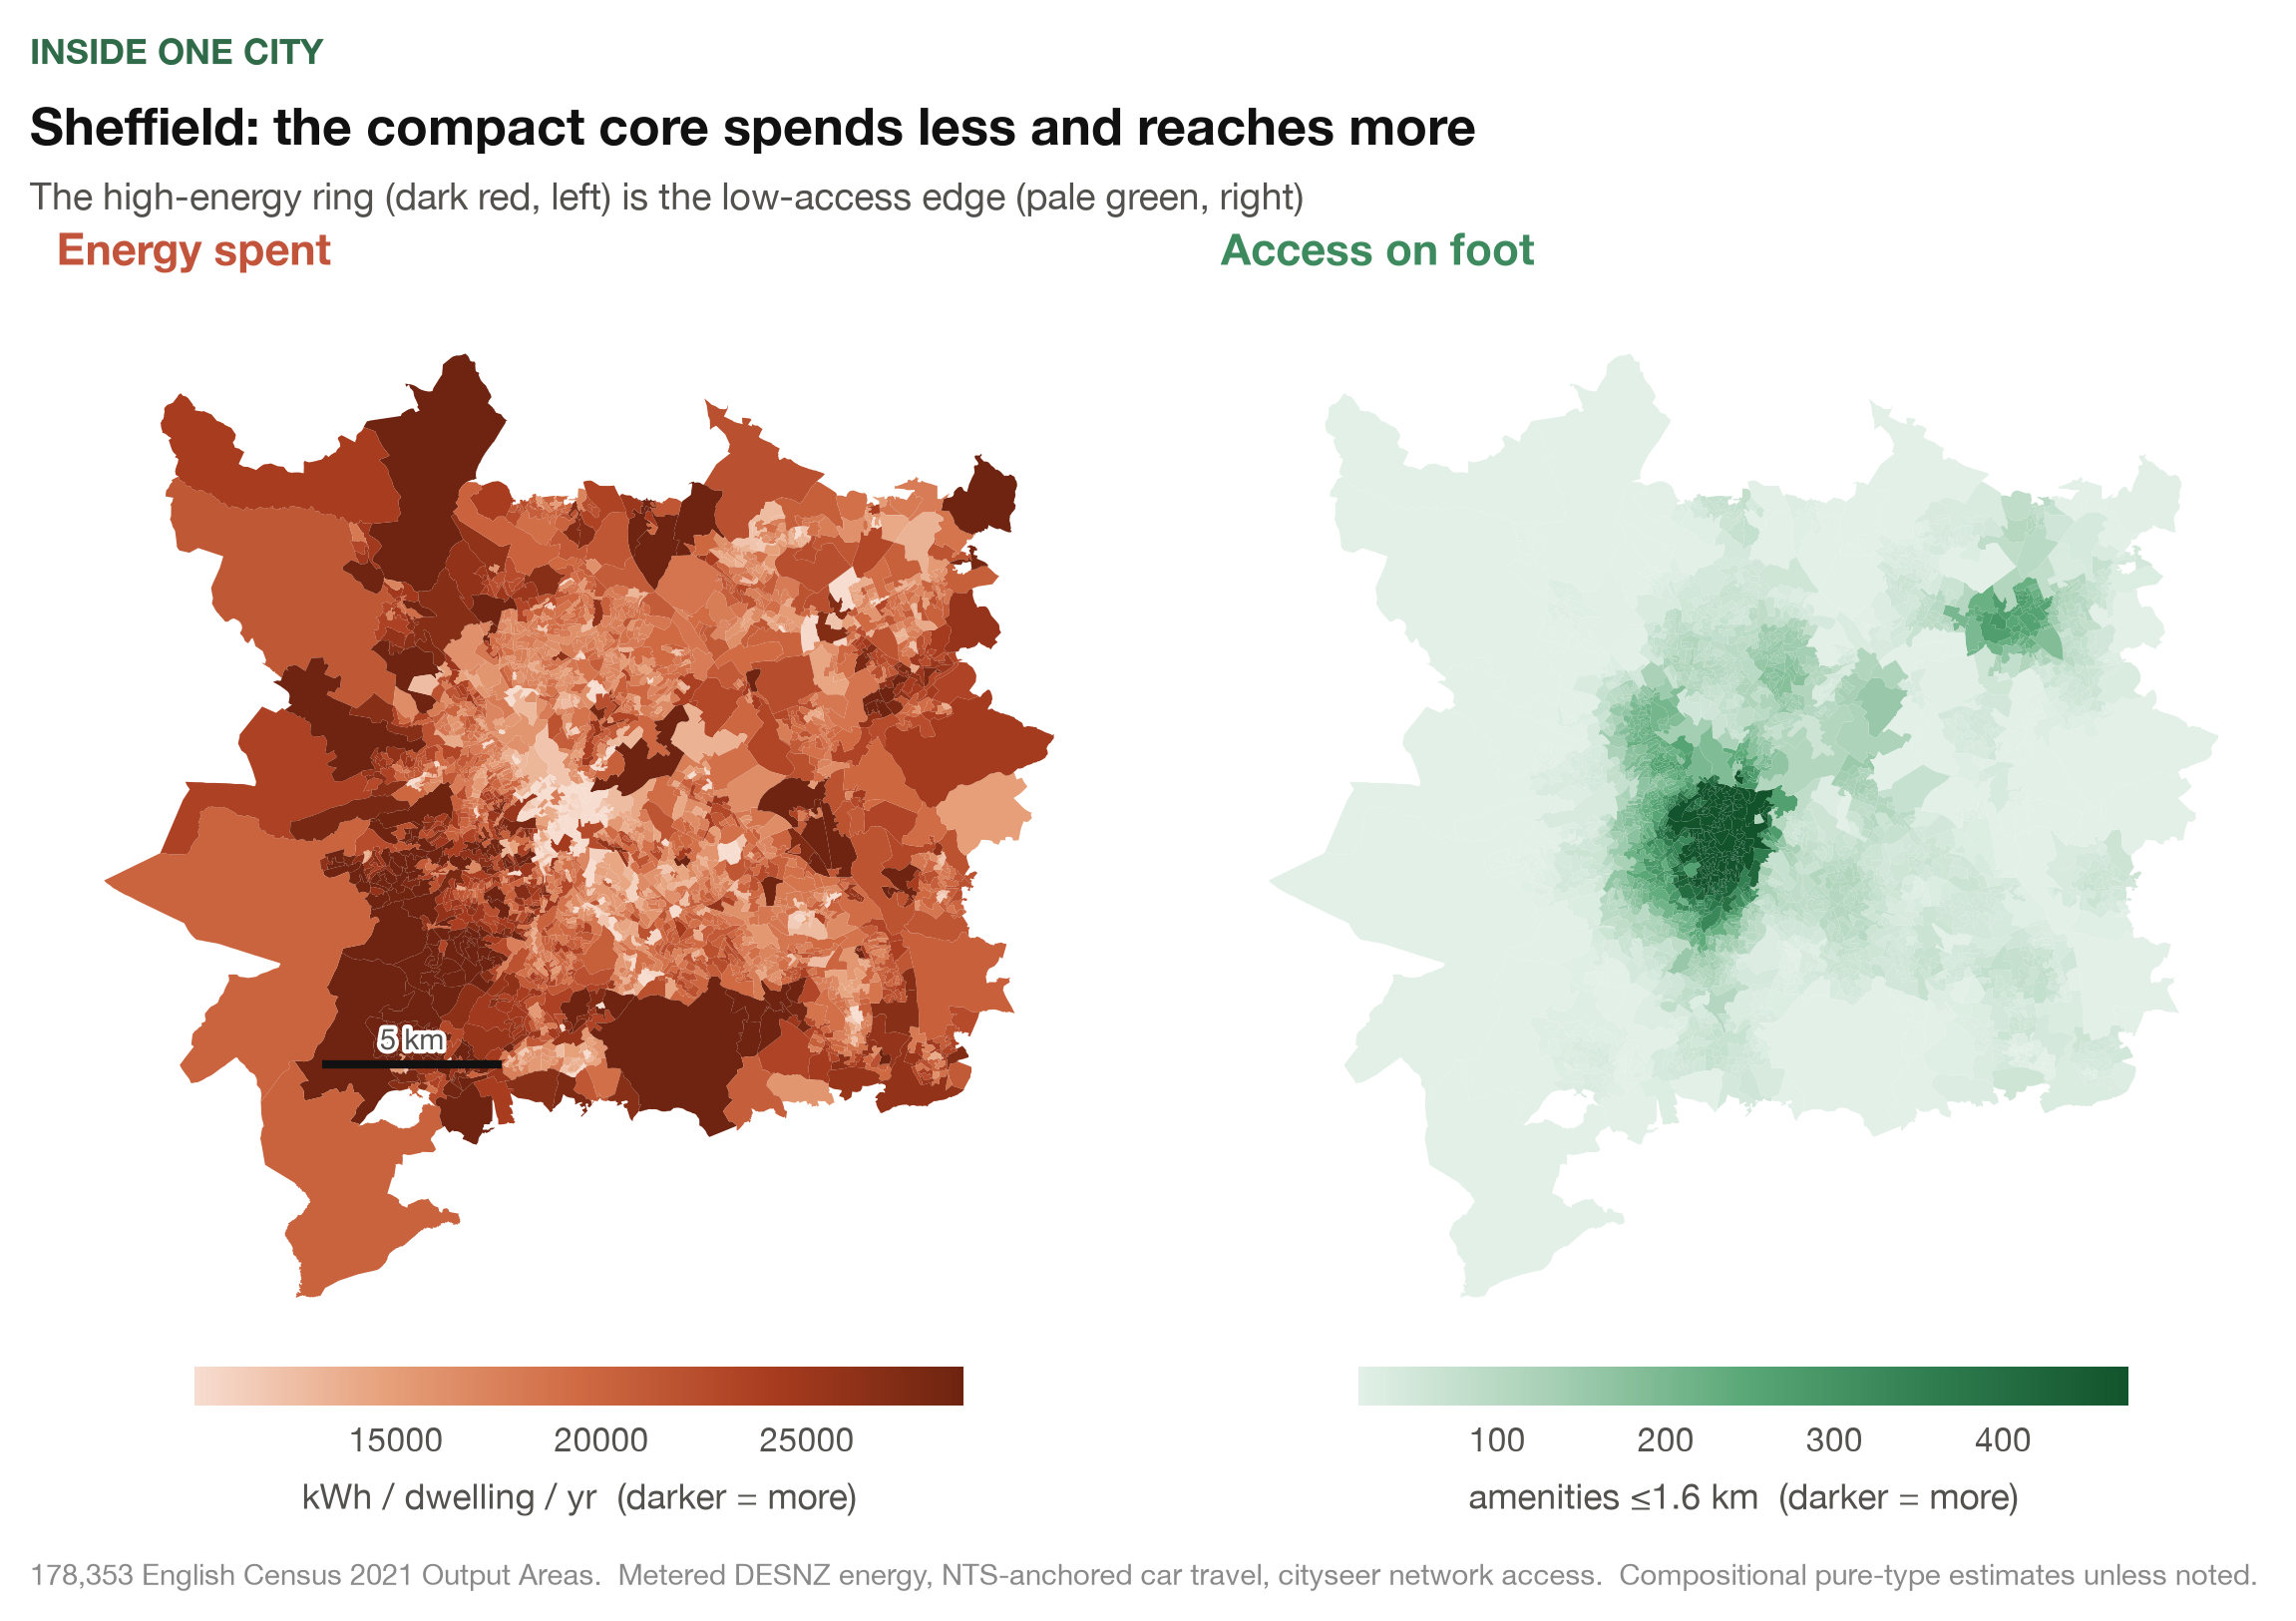
\includegraphics[width=\textwidth]{fig10_city.png}
\caption{\textbf{The two axes within a single city.} Sheffield is mapped by energy per dwelling (left) and amenities within a 1.6\,km walk (right). The high-energy ring around the compact core coincides with the areas of lowest walkable access. Colour scales are clipped at the 5th--95th percentiles.}
\label{edfig:city}
\end{figure}

\begin{table}[p]
\caption{Amenity destination layers: sources, record counts and filters (England; the greenspace layer is Great Britain, clipped by the Output Area extent). The six amenity types are summed into the amenity count; jobs and people are measured separately. Hospitals are excluded because the NHS trust-site register lists every site of every trust (wards, clinics, community units) rather than hospitals as such, so its count is not a credible amenity measure.}
\label{edtab:sources}
\begin{tabular}{llrl}
\toprule
Destination & Source & Records & Filter \\
\midrule
GP surgeries & NHS ODS (\texttt{epraccur}) & 12,664 & active GP practices \\
Pharmacies & NHS ODS & 11,268 & community pharmacies \\
Schools & GIAS & 50,631 & open establishments \\
Food outlets & FSA hygiene register & 190,359 & restaurants, cafes, takeaways, pubs \\
Food shops & FSA hygiene register & 93,071 & supermarkets and convenience retail \\
Parks and greenspace & OS Open Greenspace & 102,773 & parks, playing fields, play spaces, allotments \\
Jobs & Census 2021 WP101EW & --- & workplace jobs, weighted by job count \\
People & Census 2021 TS001 & --- & resident population \\
\botrule
\end{tabular}
\end{table}

\begin{table}[p]
\caption{The decarbonisation-scenario ladder with 95\% confidence intervals (compositional detached:flat total energy per dwelling, clustered on local-authority districts). The equal-household-size column holds log household size as a freely estimated control. Every scenario is fitted on the common complete-case sample of \nepiscenarioN{} areas. The Balanced Pathway estimate is insensitive to the assumed heat-pump seasonal coefficient of performance (\nepicopLow$\times$ at 2.4, \nepicopMid$\times$ at 2.8, \nepicopHigh$\times$ at 3.2).}
\label{edtab:scenarios}
% Generated by the stats scripts via stats/ledger.py — do not edit.
% Regenerate by running the stats scripts (see paper/submission_checklist.md).
\begin{tabular}{lcc}
\toprule
Scenario & Unadjusted [95\% CI] & Equal household size [95\% CI] \\
\midrule
Status quo & 2.11$\times$ [2.00, 2.23] & 1.70$\times$ [1.61, 1.80] \\
Insulation only (100\%) & 1.82$\times$ [1.74, 1.91] & 1.46$\times$ [1.38, 1.54] \\
Heat pumps only (100\%) & 2.16$\times$ [2.08, 2.24] & 1.79$\times$ [1.70, 1.88] \\
Electric vehicles only (100\%) & 1.84$\times$ [1.71, 1.98] & 1.47$\times$ [1.37, 1.58] \\
Insulation + electric vehicles (100\%) & 1.50$\times$ [1.42, 1.58] & 1.17$\times$ [1.11, 1.24] \\
CCC Balanced Pathway 2040 & 1.88$\times$ [1.79, 1.97] & 1.51$\times$ [1.44, 1.59] \\
Full rollout (100\%) & 1.67$\times$ [1.61, 1.73] & 1.35$\times$ [1.29, 1.42] \\
\botrule
\end{tabular}

\end{table}

\begin{table}[p]
\caption{Self-selection robustness. Treatment is the continuous detached share (0$\to$100\%) in an OLS specification with an intercept, over all areas; confounds are building age, deprivation (overall index and income domain), tenure and heating-degree-days; NS-SeC (National Statistics Socio-economic Classification) adds the higher managerial and professional occupational share. $\delta^{*}$ is the Oster (2019) coefficient-stability bound with $R_{\max} = \min(1.3\tilde{R}, 1)$; the final column is the bias-adjusted gap at $\delta = 1$. The small bound for home energy indicates that the home-energy gap alone does not survive selection comparable to the observed confounds; the argument accordingly rests on access and the rate.}
\label{edtab:oster}
% Generated by the stats scripts via stats/ledger.py — do not edit.
% Regenerate by running the stats scripts (see paper/submission_checklist.md).
\begin{tabular}{lccccc}
\toprule
Outcome & Raw & + confounds & + NS-SeC & Oster $\delta^{*}$ & Adjusted at $\delta = 1$ \\
\midrule
Total energy & 1.87$\times$ & 1.29$\times$ & 1.29$\times$ & 1.15 & 1.03$\times$ \\
Home energy & 1.30$\times$ & 1.03$\times$ & 1.02$\times$ & 0.37 & 0.95$\times$ \\
\botrule
\end{tabular}

\end{table}

\begin{table}[p]
\caption{Scale sensitivity (modifiable areal unit problem). The identical compositional model re-fitted after household-weighted aggregation to the two coarser census geographies, with 95\% LAD-clustered confidence intervals, alongside the support-respecting dominant-type median ratios. The home-energy vertex contrast attenuates toward parity at MSOA scale, with a confidence interval spanning one, because almost no MSOA approaches a pure dwelling-type composition; the median counterpart remains above one at every scale.}
\label{edtab:maup}
% Generated by the stats scripts via stats/ledger.py — do not edit.
% Regenerate by running the stats scripts (see paper/submission_checklist.md).
\begin{tabular}{lrcccc}
\toprule
Scale & Units & Home [95\% CI] & Total [95\% CI] & Home (medians) & Total (medians) \\
\midrule
Output Area & 178,322 & 1.59$\times$ [1.45, 1.76] & 2.11$\times$ [2.00, 2.23] & 1.47$\times$ & 1.74$\times$ \\
LSOA & 33,742 & 1.17$\times$ [1.02, 1.33] & 1.87$\times$ [1.73, 2.02] & 1.32$\times$ & 1.59$\times$ \\
MSOA & 6,855 & 0.91$\times$ [0.76, 1.09] & 1.71$\times$ [1.54, 1.91] & 1.17$\times$ & 1.47$\times$ \\
\botrule
\end{tabular}

\end{table}

\end{document}
